\chapter{Floods and Droughts: Thailand}
\chapterauthor{Celine Liu, Heng Jia Min, Jeffrey Tong, Nathalie Baer Chan, and Sonia Kaur Sambhi\footnote{Contribution Statement: All authors contributed equally to the paper in the form of research, writing, section editing and compilation of the bibliography and all sources. All authors were assigned to work on 2 chapters each. CL worked to put together the Introduction and Chapters 2 and 4. HJM worked to assemble Chapters 1, 2 and 6. JT worked on Chapters 3 and 5. NBC worked on Chapters 3 and 4. SKS worked on Chapters 5 and 6. JT worked on overall edits for style, language and logical flow to ensure consistency and comprehensibility of the final document.}}

\section{A Cycle of Floods and Droughts in Thailand}

From July to December 2010, as the rainy season reached its peak across Thailand, floodwaters from the north began inundating the central provinces, threatening to head south into Bangkok in what would turn out to be the worst flood disaster to hit Thailand in half a century (Gale \& Saunders, 2015). Just months before this incident, Thailand was still in the midst of battling its most serious drought in decades (Garbero, 2013). 

This cycle of floods and droughts, a common feature of life in Thailand, may seem puzzling given Thailand’s annual rainfall far exceeds its annual water demand, according to Sumet Tantivejkul, Utokapat Foundation chairman. During the Sustainable Water Management Forum 2016, Tantivejkul highlighted, ``[Thailand receives] around 754,000 million cubic metres of rain per year. That is more than enough for the annual water demand of around 100,000 million cubic metres\ldots However, only 5.7\% of rainfall, 70,370 million cubic metres, empties into the reservoirs.''

However, how floods and droughts arise are less to do with the volume of precipitation than the uneven distribution of precipitation across timescales and geographical locations, especially as it relates to the El Nino Southern Oscillation and the Indian Ocean Dipole. These distribution patterns interact with Thailand’s water resource management approaches such as dams and water use to, resulting in floods and droughts of varying severity.

\begin{figure}
	\centering
		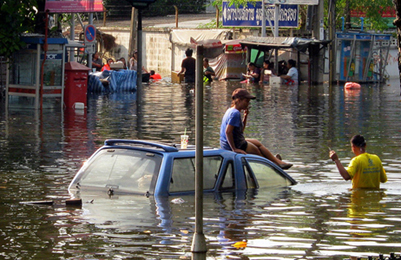
\includegraphics[width=0.50\textwidth]{Flood_Thailand.jpg}
	\caption{Figure 1: Floodwaters reach waist deep during the 2011 Thai Floods (Source: TBD).}
	\label{fig:Flood_Thailand}
\end{figure}


\section{Mechanisms of Floods and Droughts}

Floods are generated when a stream’s discharge exceeds the capacity of its channel, resulting in water inundating land that is normally dry. There are three main types of floods: coastal (surge) floods, pluvial (surface) floods and fluvial (river) floods. Coastal floods are caused by the inflow of saltwater (usually the result of a large storm or tsunami) from the ocean to inland areas, while pluvial and fluvial floods are caused by the runoff of water from the land, usually during excessive rain or sometimes ruptured dams (Maddox, 2014). 

Floods take hours or even days to develop. When there is rain, stream discharge gradually increases until it reaches a peak flow. Floods emerge when the stream discharge crosses a particular threshold (determined by the channel’s capacity), and can be categorised as flash floods when the time lag between intense rainfall and peak flow is very small (Figures 2 and 3; Skinner and Murck, 2011). Stream discharge is the product of the velocity, depth and width of water flowing through it. Channel capacity can be modelled by different equations, but Manning’s equation (1891) which applies to uniform flow in open channels is commonly used:

\begin{equation}
Q = VA = (\frac{1}{n})AR^{2/3}\sqrt{S}
\end{equation}
 
\noindent Where (in SI Units):

\begin{itemize}
	\item Q = Flow rate (m3/s)
	\item V = Velocity (m/s)
	\item A = Flow area (m2)
	\item n = Manning’s roughness coefficient (s/m1/3)the higher the coefficient, the greater the resistance to flow)
	\item R = Hydraulic radius (m)
	\item S = Channel slope (unitless)
\end{itemize}

Floods are classified based on their theoretical likelihood of occurring in a given time period. For example, a large destructive flood that is expected to happen only once every century is classified as a hundred-year-flood. What this theoretical likelihood translates to, in reality, is a one-percent chance that such a flood would happen in any given year. Unlike tectonic hazards, the occurrence of a flood of great magnitude does not reduce the probability of a flood of similar magnitude happening in the next year. Instead, after one flood season, the extensive ground saturation may make it even more difficult for water to infiltrate, increasing the likelihood of a flood in the next flood season (United States Geological Survey, 2018). 

\begin{figure}[htb]
	\centering
		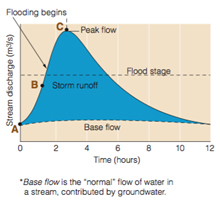
\includegraphics[width=1.00\textwidth]{graphics/base_flow.jpg}
	\caption{Hydrograph representation of the formation of floods (Source: Skinner and Murck, 2011).}
	\label{fig:base_flow}
\end{figure}
 
\begin{figure}[htbp]
	\centering
		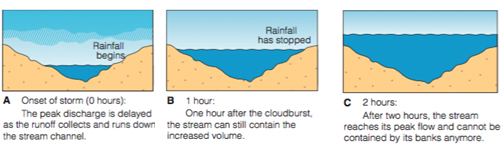
\includegraphics[width=1.00\textwidth]{graphics/hydrograph.jpg}
	\caption{Figure 3: Visual representation of flood formation in a waterway (Source: Skinner and Murck, 2011).}
	\label{fig:hydrograph}
\end{figure}
  

Drought as a physical phenomenon is difficult to define, as over 150 published definitions of drought in the 1980s (National Drought Mitigation Center (U.S.), 2018) might testify to. Wilhite and Glantz (1985) have classified the definitions into four approaches: meteorological, agricultural, hydrological, and socio-economic. Meteorological drought, which defines drought on the basis of a degree of dryness in comparison to an expected, normal amount, is what most researchers and articles refer to when discussing drought. Meanwhile, agricultural drought refers to drought as it relates to agriculture, such as its effects on plant water demand, soil water deficits, reduced groundwater, or topsoil moisture levels. Hydrological drought, which can lag behind meteorological and agricultural drought, concerns precipitation deficiencies in particular components of the hydrological system, such as groundwater and reservoir levels, streamflow and soil moisture. Socio-economic drought approaches then define drought with reference to demand and supply, such as Hoyt’s definition (1936) of drought as occurring “when precipitation is not sufficient to meet the needs of established human activities”. 

While we broadly refer to drought as a physical phenomenon arising from lower-than-average rainfall (meteorological drought) in this paper, we acknowledge that other definitions of drought contribute to the significance of drought to Thailand as well. For example, agricultural drought is important for Thailand where agriculture contributes 8-10\% of its GDP every year (The World Bank, 2018), and where droughts can contribute to as much as 20 billion baht (634.3 million USD) losses in purchasing power among farmers, as in the case of the 2016 flood crisis (Thaiturapaisan, 2016). Hydrological drought is concerning given the 25 river basins and 254 sub-basins that Thailand possesses (The World Bank, 2011), which result in downstream effects that cannot be accounted for merely by local precipitation levels. Finally, socio-economic drought is concerning particularly for a country whose water demand is likely to continue increasing with urbanisation and economic development (The World Bank, 2011).

Interestingly, the probability of drought can increase following a flood, by disturbing the ability of water buffers to store the excess water as a water source during water-scarce periods. For example, during periods with normal levels of precipitation, water can infiltrate the ground as groundwater, but during a flood most of the precipitation enters the sea directly as runoff. Over time, the reduced groundwater supply can contribute to agricultural drought.

\section{Flood and Drought Meteorology}

\subsubsection{General Precipitation Trends}

Thailand is located between latitudes 6 and 20 degrees north. Its southern region experiences an equatorial climate with even rainfall throughout the year. Central and northern regions are characterized by a tropical monsoon climate with more clearly defined dry and wet seasons. 

\begin{figure}[htbp]
	\centering
		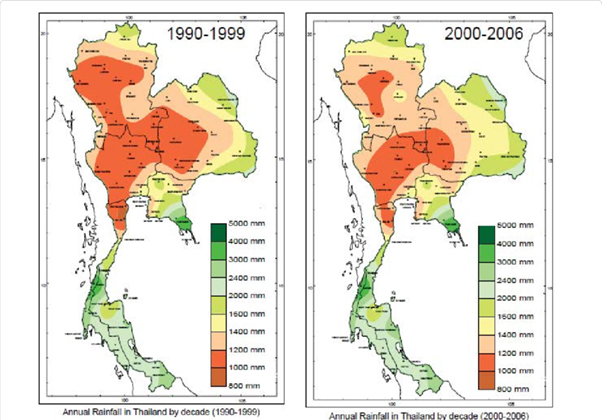
\includegraphics[width=1.00\textwidth]{graphics/Annual_Rainfall_Thailand.jpg}
	\caption{NOTE: Find better reference than this one.}
	\label{fig:Annual_Rainfall_Thailand}
\end{figure}

In particular, the climate of Thailand may be divided into three seasons as followed (Meteorological Department of Thailand):  

\begin{itemize}
	\item Rainy or southwest monsoon season (mid-May to mid-October). The southwest monsoon prevails over Thailand and abundant rain occurs over the entirety of the country, with 80\% of the average annual rainfall occurring during this period. During the wettest months of August and September rivers carry high runoffs and can overflow, leading to flooding (Figure 4). In extreme rainfall years the flooding may spread along Thailand's main water artery, the Chao Phraya River basin, towards Bangkok, the country's capital, before emptying into the sea.

\item Winter or northeast monsoon season (mid-October to mid-February). This is the mild period of the year in northern Thailand but the wettest point in the Southern East Coast, especially during October to November.  

\item Summer or pre-monsoon season (mid-February to mid-May). This is the transitional period from the northeast to southwest monsoons (Figure 4). The weather becomes warmer, especially in northern Thailand. Droughts are prevalent in the north during this period, while the south is generally protected due to its equatorial climate and more even rainfall.
\end{itemize}

\subsection{Periodic Sea Surface Temperature Cycles and Precipitation}

These annual weather patterns may also be exacerbated or moderated by periodic cycles such as the El Niño Southern Oscillation (ENSO) and Indian Ocean Dipole (IOD).

ENSO is an irregular periodic variation in winds and sea surface temperatures over the tropical eastern Pacific Ocean. The warming and cooling phases of sea temperature changes are known as El Niño and La Niña respectively. The two periods last several months each (typically occurring every few years) and their effects vary in intensity. In Southeast Asia, the impact from La Ni\~na is typically wetter-than-normal rainfall conditions, especially during the Southwest Monsoon period (June-September). In contrast, during El Niño years, the region generally experiences less-than-normal rainfall. This trend, however,  is especially inconsistent within Thailand (see Figure 5). 

However, Buckley, B. et. al (2007) claim evidence for the long-term influence of ENSO on the variability of the Northern Thailand monsoon, and suggest that El Niño conditions significantly contribute to drought in the region. Using a multi-sample teak tree-ring chronology, they discovered the occurrence of two periods of greatly diminished rainfall in the 1700s, corresponding to periods of anomalously warm sea surface temperature (SST) in the central and eastern tropical Pacific. 

More research needs to be conducted in this area to determine the true effects of ENSO on precipitation in Thailand.

\begin{figure}[htbp]
	\centering
		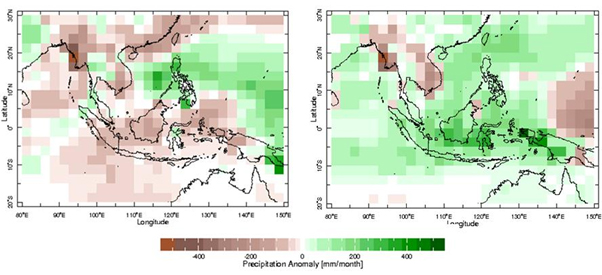
\includegraphics[width=1.00\textwidth]{graphics/Rainfall_Anomly_Thailand.jpg}
	\caption{June to October rainfall anomaly composite for El Niño years (left) and La Niña years (right) between 1979 and 2016. Note that particularly in Thailand, El Niño years do not necessarily correlate with lower precipitation and vice versa. However, a general trend across most of Southeast Asia still remains.}
	\label{fig:Rainfall_Anomly_Thailand}
\end{figure}

Likewise, the Indian Ocean Dipole (IOD) is an irregular oscillation of sea-surface temperatures in which the western Indian Ocean becomes alternately warmer and then colder than the eastern part of the ocean. A negative phase sees greater-than-average sea-surface temperatures and greater precipitation in the eastern Indian Ocean region (such as in Thailand), with a positive phase having the opposite effect (Figure 6). An average of four positive-negative IOD events occur during each 30-year period with each event lasting around six months (Saji and Yamagata, 2003).

\begin{figure}
	\centering
		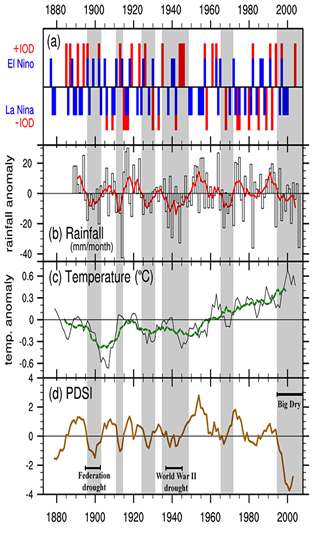
\includegraphics{ENSO2.jpg}
	\caption{Caption and Source needed}
	\label{fig:ENSO2}
\end{figure}


Chansaengkrachang et al. (2011) report that strong negative (positive) IOD may cause higher (lower) Thai rainfall in corresponding months based on 1979–2008 monthly rainfall observations. However, the study observed a weaker correlation (overall r = 0.11) than that found with the following year's summer monsoon (r = 0.31–0.38) indicating a delayed association (Bridhikitti, A., 2012).

\begin{figure}[htbp]
	\centering
		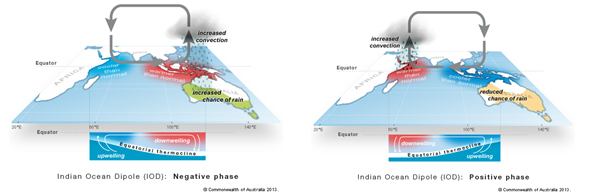
\includegraphics[width=1.00\textwidth]{ENSO3.jpg}
	\caption{Effects of the Indian Ocean Dipole on Temperature and Precipitation}
	\label{fig:ENSO3}
\end{figure}


These periodic sea surface temperature cycles may interact and either exacerbate or moderate one another in any given period of time. Both must be taken into account in order to determine their combined effect on precipitation.

\subsection{Climate Change and Long Term Precipitation Trends}

According to Marks (2011), climate change in Thailand will likely take three forms: (1) increased mean daily maximum temperatures in Thailand by as much as 1.9 degrees Celsius by 2050 (The World Bank, 2009), (2) a continued decrease in the number of rainy days (Sharma, 2014), and (3) precipitation events (storms and floods) that, while short, are intense and destructive (Anthes et al., 2006; Dasgupta et al., 2009). Meanwhile, the exact impacts of climate change on tropical cyclones, ENSO events and the Asian monsoon are indeterminate (Singhrattna et al., 2005). East and Central Thailand will observe decreases in total rainfall, while the Northeast and Gulf region, together with the Bangkok metropolitan area, are likely to experience increasing rainfall (Naruchaikusol, 2016; Limsakul \& Singhruck, 2016).

Sea level rise is one significant effect of these climatic changes. The Gulf of Thailand has been rising a quarter of a centimetre every year. With the low elevation of coastal regions (which are an average of only a metre above sea level), (Marks, 2011) and land subsidence exacerbated by intensive groundwater use, Bangkok along with the rest of Central Thailand along the coast is likely to suffer prolonged flooding. The coastal floods that result from sea level rise will also result in higher salt levels in the soil (saline intrusion) (South East Asian -- Global Change System for Analysis, Research and Training, 2009).

Recall the example of the 2010 drought and 2011 flood in the introduction of this chapter (more details in Box 1). In the 2010 drought, the Mekong River water level was sufficiently low that villagers shared how they could sometimes walk across the river -- an event which ‘has never happened before’ (Leitsinger, 2010). The above weather patterns of the annual and interannual distribution of precipitation have become more unpredictable as a result of climate change, resulting in the increasing likelihood of rare events.


\section{The Geography of Floods and Droughts in Thailand}

This section explores the geographical distribution of flood and drought events, and examines their implications on the lives of individuals potentially vulnerable to such hazards.

\subsection{Spatial Distribution of Floods}

Rainfall patterns, elevation and local infrastructure significantly determine the location of flood events in Thailand. The densely populated lowland regions of Thailand, including the Bangkok Metropolitan Region, most notably contain the outlets of major river basins which drain water from the northern, higher-elevation regions of the country. Along coastal regions, tidal floods from the Gulf of Thailand and stormwater from local rainfall simultaneously contribute to the production of floodwaters.

Examining the Chao Phraya River Basin in detail reveals the vulnerability of the capital and primate city of Bangkok: the city sits not only at the confluence of multiple streams originating from the highland regions of Northern Thailand, but is also located along the coast where tidal floods from the Gulf of Thailand may prevent basin drainage. Most of the city is located in the floodplains slightly above mean sea level on both banks of the river (Figure 8) (Klongvessa \& Chotpantarat, 2014; Sayama et al., 2017). Simulations based on rainfall data, topography and satellite imagery reveal that flooding in the Chao Phraya River Basin is predicted to occur most severely within Bangkok and lower Nakhon Sawan -- regions with the greatest flood depths (Figures 8 and 9) (Sayama et al., 2017).

\begin{figure}[htbp]
	\centering
		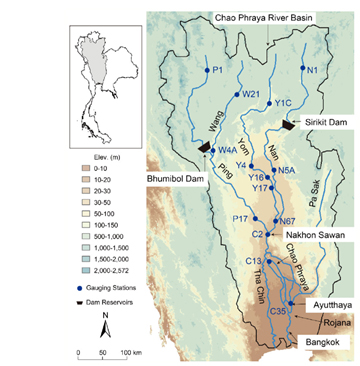
\includegraphics[width=1.00\textwidth]{Chou_Phraya_Basin_Thailand.jpg}
	\caption{Map of the Chao Phraya River Basin (Sayama et al., 2017)}
	\label{fig:Chou_Phraya_Basin_Thailand}
\end{figure}

\begin{figure}[htbp]
	\centering
		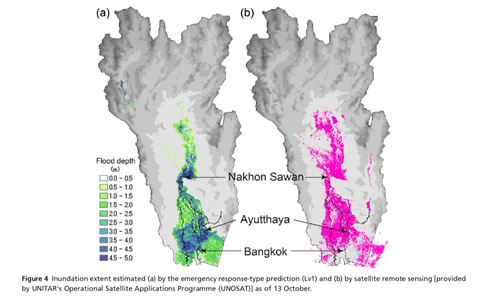
\includegraphics[width=1.00\textwidth]{graphics/Flood_Depth_Simulation_Thailand.jpg}
	\caption{Flood Depth Simulation in the Chao Phraya River Basin based on rainfall data and predictions, river basin characteristics (which include evapotranspiration, dam outflow and storage volume, tidal effect, river cross section), and elevation (Sayama et al., 2017)}
	\label{fig:Flood_Depth_Simulation_Thailand}
\end{figure}

Furthermore, flood depths could also be potentially increased by land uses which further exacerbate land subsidence. Owing to historic groundwater extraction and pumping, land subsidence has been most prominent in the regions within and immediately surrounding Bangkok. The rate of subsidence in the capital, however, has consistently decreased (from 1 to 2 cm/year from 1978-2007 to approximately 0.97cm/year currently) due to government efforts to curb groundwater extraction (Poonam et al., 2010). The average rate of land subsidence is further predicted to decrease by 10\% per year assuming the continuity of efforts. (Poonam et al., 2010). Despite such interventions, subsidence is still expected to occur, with increasingly greater proportions of the Bangkok Metropolitan Region found at lower elevations by 2050 (Poonam et al., 2010). The predicted inundation area within Bangkok and neighboring Samut Prakarn during a 1-in-30 year flood, for instance, is expected to increase from 550 km2 (2008) to 734 km2 in 2050 (Poonam et al., 2010). 

A particular region of interest that has experienced the most severe flood events is the province of Chachoengsao to east of Bangkok. The province is host to the largest land area of inland shrimp farms in Thailand, with more than 8000 shrimp farms and 29,157 shrimp ponds (Seekao \& Pharino, 2016). However, shrimp farms in the province have been vulnerable to frequent flooding: Chachoengsao sits in the low-elevation Bangpakong River Sub-Basin and is located downstream of the confluence of Prachinburi and Nakhonnayok Rivers. As a consequence, floodwaters in 2011 for instance have severely inundated shrimp farms in the region, contributing to shrimp farm economic losses of approximately 109 million Baht (US\$3.41 million) nationally (Seekao \& Pharino, 2016). Researchers also note that the province has recently experienced repeated flooding almost annually, and highly vulnerable areas correlate with the areas most severely inundated by floodwaters in 2011 (Seekao \& Pharino, 2016). Flood vulnerability maps for the region and its aquaculture industry, however, remain scarce, while information about local vulnerability has been limited and inadequately communicated to farmers in the region (Seekao \& Pharino, 2016). 

\subsection{Spatial Distribution of Droughts}

Due to the diverse topography and geography of the land, certain areas of Thailand are naturally prone to periods of delayed rainfall and water shortage, particularly under global climate conditions of increasing stochasticity. However, the majority of drought damage is caused by the geopolitical distribution of water rather than the quantity itself, as suggested by the lack of correlation between rainfall maps and disaster occurrence (Figure 10). In fact, drought incidence is a function of numerous factors including humidity, soil moisture, length of drought, drought area, drainage basin, land use, and water infrastructure. In recent years, interplay between the latter two factors has led to increased drought vulnerability, as residential areas, economic activities, and agriculture have expanded beyond the capacity or physical reach of existing irrigation systems (UN-Water Country Report, 2014). 

\begin{figure}[htbp]
	\centering
		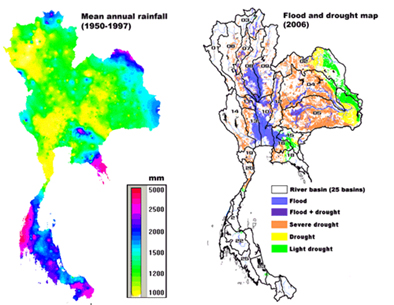
\includegraphics[width=1.00\textwidth]{graphics/Rain_Hazards_Thailand.jpg}
	\caption{Comparison between mean annual rainfall and the incidence of floods and droughts (Chitradon, 2009).}
	\label{fig:Rain_Hazards_Thailand}
\end{figure}

Thailand is often discussed with reference to four distinct geographic regions -- Northeast, North, Central, and South -- that experience water insecurity according to the vulnerabilities created or exacerbated by land use, unequal infrastructure investments, and water consumption. The Northeast is characterized by mountains, the large Khorat plateau, the Mekong River, and grasslands, and is substantially less industrialized than the rest of the country (Geography of Thailand, 2014). Although the typically arid Northeast receives a medium-high volume of rainfall during the wet season and even floods in its river basins, existing water infrastructure developments including dams frequently fail to sustain sources through the extensive dry season, when the area’s water basins diminish by around 82\% (UN-Water Country Report, 2014). Bordering this region is the North, whose Ping, Wang, Yom, Nan river basins hold much more fertile soils that the Northeast and are generally less drought-prone, but were hit hardest during the 2016 droughts (Fox, 2016). This may be because of the quantity of water-intensive agricultural activities in the North as well as the water security disparity between irrigated and non-irrigated lands (UN-Water Country Report, 2014). Similarly, the fertile Central region’s Chao Phraya basin has many irrigated lands and development projects due to the commercial success of Bangkok, but intense rice paddy cultivation and other industries have increased Central Thailand’s water demand above its dry season capacity (Geography of Thailand, 2014). The Southern region experiences the heaviest annual rainfall in the country, but due to lacking infrastructure and intensive farming can lose up to 85\% of its water at its driest (UN-Water Country Report, 2014). 

\begin{figure}[htbp]
	\centering
		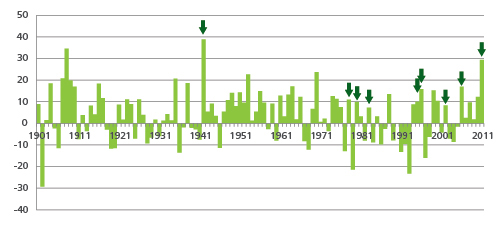
\includegraphics[width=1.00\textwidth]{graphics/Water_demand_Thailand.jpg}
	\caption{Is this water demand? by month? year? Put axis labels, reference (see above…)}
	\label{fig:Water_demand_Thailand}
\end{figure}

Of Thailand's land area of 510,890 sq km, only 64,150 sq km of land were irrigated as of 2012, leaving 87\% of the country without reliable water sources, including a significant portion of its farmland (CIA World Factbook). However, even in the most irrigated lands, dramatic increases of industrial water use threaten the agricultural sector and consequently the Thai economy (Thaiturapaisan, 2015). 

\begin{figure}[htbp]
	\centering
		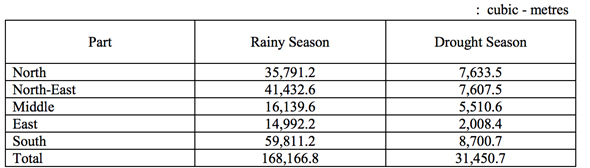
\includegraphics[width=1.00\textwidth]{graphics/Water_volume_by_season_Thailand.jpg}
	\caption{Average Annual Quantity of Water in Regional River Basins in Thailand (Source: Draft of Master Plan About Drought in Thailand)}
	\label{fig:Water_volume_by_season_Thailand}
\end{figure}


\begin{figure}[htbp]
	\centering
		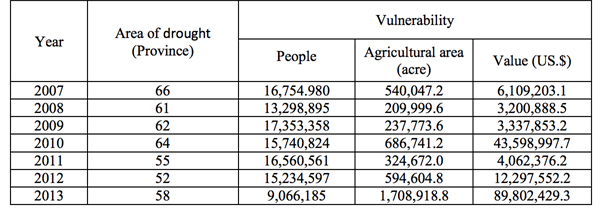
\includegraphics[width=1.00\textwidth]{graphics/Drought_vulnerability.jpg}
	\caption{Statistics of Major Droughts between 2007 and 2013 (Source: Department of Disaster Prevention and Mitigation)}
	\label{fig:Drought_vulnerability}
\end{figure}

\section{The Politics of Floods and Droughts in Thailand}

Within the context of Thailand, political actions and contestations by multiple agents play significant roles in determining the outcomes of disaster preparedness, response, water resource management, and mitigation. We explore in this section the influence politics has had in the management of floods and droughts.

\subsection{An Overview of Thai Politics and History}

Thailand is unique in Southeast Asia as the only country with no colonial past, maintaining an absolute monarchy system until 1932. Following this, it saw sixty years of military rule before the first democratic coup of 1973, which kickstarted a series of successive oscillations between military and civilian governments. In total, Thailand has had 25 general elections and 19 coups d'état since 1932, with 12 of them successful. At the same time, the monarchy remains deeply influential despite their limited constitutional power. As such, the politics of power hangs in a precarious balance between three main actors -- the military, the civilian government and the monarchy -- and this instability has undermined efforts to establish an effective disaster risk management policy. 

\subsection{The Influence of Political Instability of Water Infrastructure and Disaster Incidence}

Flood and drought management is currently fragmented across various ministries and agencies such as the Royal Irrigation Department (RID), the Electricity Generating Authority of Thailand (EGAT), the Meteorological Department, the Department of Water Resources (DWR), the National Disaster Warning Centre (NDWC), the Ministry of Public Health (MPH) etc. In 2011, the Office of National Water and Flood Management Policy (ONWF) was created within the Yingluck cabinet in response to the 2011 floods to harness the water-related competences of the various state agencies and focus on effective and coordinated management of water-related disasters. 

Yet the future of this agency is now uncertain following the ousting of the cabinet in the 2014 coup (Maier-Knapp, N., 2015). Inter-institutional rivalry and the lack of cross-agential coordination has led to coordination efforts in Disaster Risk Management to be negligible among state agencies (Shook, 1997; Huaisai et al., 2006; Foran et al., 2012), and efforts to address these concerns have been threatened by political instability. Failing to address these concerns may exacerbate individual vulnerability to water-related hazards.

\subsubsection{Disaster Preparedness} 

In light of heavy bureaucracy and political instability, basic disaster preparedness systems remain ineffective. Thailand’s Meteorological Department has long complained of an inadequate rainfall prediction system; with regards to the 2011 floods, department authorities stated that, “No one expected rainfall would be this much. Right now our system, including hardware and software, is obsolete.” Requests for a 4 billion baht (\$130 million) overhaul of its radar and modeling systems had gone unheeded since 2009 (Bloomberg, 2011). Smith Dharmasaroja, former director general of the Thai Meteorological Department, highlights that these miscalculations were directly responsible for exacerbating the floods, as water from the dams were forced to be discharged too late during the height of the disaster.

Furthermore, the tense history and relationship between the military and civilian government has undermined disaster warning systems as local authorities are cautious in declaring disasters or dispatching military personnel as an initial response (Setboonsarng, 2011). If armed forces are deployed immediately, this signals a security response to the population and implies higher levels of emergency. In addition to this, sending armed forces into areas of ongoing conflict is a delicate matter that could aggravate the conflict-torn provinces in the more vulnerable south. This is despite the fact that disaster management efforts are ultimately dependent on the military due to their resources and experience (Maier-Knapp, 2015). 

In 2017, the northern province of Sakon Nakhon was hit with the worst flooding in 20 years, affecting 426,000 people and killing at least 7. Reportedly, warnings by local authorities were contradictory and confusing; at the peak of the flood, pictures of the overflowing Huai Sai Khamin reservoir were posted on social media and quickly dismissed by the Irrigation Department, while the Department of Disaster Prevention and Mitigation continually denied local reports of malfunction with an emergency siren warning tower (Bangkok Post). 

\subsubsection{Disaster Response and Recovery}

In times of disaster, political instability and inefficiency further worsens response during the most critical moments, as conflicting parties with different agendas compete over management strategies. 

Presently in Thailand, divide between the interests of the rural and urban areas manifest themselves along party lines, leading to conflicts between the central government, which relies heavily on rural support, and opposition parties, which have strong support in urban centres. This may lead to competing agendas during disaster events. During the 2011 floods, clashes between the Bangkok’s opposition-run Governor’s office and the central government were critical in determining the city’s response strategies. When the central government ordered a redirection of flood waters towards the city centre, a bastion of support for the city’s governor, the Governor openly challenged the legality of the prime minister’s decision. This led to the delay in deploying 800,000 sandbags, which were refused by the city’s governor, and have also led to accusations of favouritism in disaster-response decisions by different levels of government (The Centre for Climate and Security). In the later days of the flood, the Governor also contradicted the official statement of safety by the Police General and Prime Minister by urging his residents to evacuate, saying, “Listen to me and only me. I will tell you when it is safe” (quoted in Setboonsarng, 2011).

The political situation in Thailand was further complicated following the re-establishment of the military government under Prime Minister Prayuth Chan-ocha in 2014, who some blame for withholding government disaster relief in the aftermath of the 2016 El Niño droughts (Lewis, 2016). Chan-ocha in fact publicly doubted the severity of the crisis and the validity of complaints from the rural authorities. He expressed in a radio address, “How can the whole province have no water?” and stressed the need for verification and prioritization of efforts based on the type of assistance required (Bangkok Post, 2016). 

Evidently, tension between the various levels and forms of political power greatly undermine efforts at creating a coherent disaster response strategy in times of crises.

\subsubsection{Disaster Mitigation}

Furthermore, anti-flood and anti-drought preventative measures can come into conflict and even outright contradict one another, forcing difficult choices on a government already stretched thin by bureaucracy and political tradeoffs. For example, management of reservoir water storage requires highly politicized decisions about when to release water from the dams, potentially wasting resources in the case of a sudden drought while increasing capacity for flood mitigation. This concurrence of floods and droughts is particularly significant due to the aforementioned lack of effective predictive technology. Retaining dam waters past the typical release point can also keep urban centres like Bangkok dry, but at the unjust expense of flooding many provinces upstream, aggravating urban/rural conflict further (Pongsudhirak, 2011). 

When floods and droughts do occur, they hit hardest in areas with the least infrastructure to prevent and minimize damage. Flood relief requires drainage systems like canal networks, and drought risk can be drastically reduced through the creation of wells; however, these property-saving industry-saving, and potentially life-saving measures can be expensive projects and are thus only installed in the densely-populated, capital-heavy urban centres of commerce. Moreover, the political instability of the early 21st century contributed to a 3.8% decline of the infrastructure construction sector in 2014 and also led to long term, large scale shortages in the workforce (BMI Research, 2015).

Dependence on hydrological infrastructure emphasizes existing contrasts and conflicts between Thailand’s economically and ecologically diverse regions, particularly between urban and rural areas. Infrastructure is a major limiting factor for urbanization, and the country is rushing to build the capacity to support its rapidly changing and modernizing economy, leaving some critics wondering how long-term these immediate response solutions could be and who they are prioritizing (Thinphanga, Thailand Environmental Institute). 

\subsection{Summary}

Political instability remains a fact of life in Thailand and the situation shows little sign of improvement, leading to a lack of a cohesive disaster management strategy. Due to the urgent nature of the natural hazard situation, many community-based, bottom-up approaches to hazard management have taken root in order to fill this vacuum. In the next section, we explore the ideologies and approaches towards disaster management that are of strong relevance to Thailand, and that could potentially advance sound disaster management policies.

\section{Ideologies and Attitudes Towards Disaster Management}

\subsection{Sufficiency Thinking and Disaster Management} 

One of the most prominent ideologies with relevance to disaster management in Thailand is Sufficiency Thinking. Thailand is the first country to adopt sufficiency thinking as a national policy, with the aim to transform the mindset of its population to “enrich everyone's lives in a truly sustainable way” (Avery \& Bergsteiner, 2016). As a form of sufficiency thinking, the Sufficiency Economy Philosophy (SEP) is a set of social, economic, environmental and cultural guidelines that has been developed by late King Bhumibol Adulyadej to build a fair, resilience and sustainable economy and society for Thailand (Box 2).

%%%%%%%%%%%%%%%%%%%% BOX 2

The SEP has been firmly anchored in Thailand’s five-year national development plans since 2002, and practical implications were evident in the 10th and 11th plans as it was stipulated that the SEP was to be applied to all parties at all levels. Innovative management practices have been applied across Thailand in agriculture, education, business, government and community organisations for over two decades (Avery \& Bergsteiner, 2016). 

In terms of disaster management, the SEP stresses the balance in the use of economic, social, environmental and cultural capital, while underlining the importance of preparedness in dealing with changes in these four dimensions (Avery \& Bergsteiner, 2016). The New Theory Agricultural Project, for instance, was introduced to lift farmers out of the vicious cycle of high debt and difficult living conditions. It is a subsistence, organic farming method which provides a step-by-step process for farmers to develop a sufficiency mindset at different levels: farmers learn to manage natural resources more sustainably while maximizing benefits to ensure food security and reduce risks from natural disasters. With a variety of crops, food and water supplies, disaster-ready buildings, and stronger community bonds, farmers are better prepared for disasters. Moreover, the lower debt and better ecological health contributes to their resilience and ability to bounce back after disasters. 

\subsection{Ecosystem-Based Disaster Risk Reduction (Eco-DRR) Approaches}

In a similar manner to the SEP, Eco-DRR is primarily an approach that emphasizes the protection and integration of natural ecosystems as disaster risk reduction measures (REFERENCE). Eco-DRR recognizes that healthy natural ecosystems, including nature reserves, mangrove forests or national parks are able to (1) offer protection or buffers against natural hazards such as floods or droughts as forms of ecosystem services, and (2) reducing the vulnerability of individuals to hazards by providing support for sustainable livelihoods and needs in the form of food, water or shelter (UNEP, 2015). Guidelines offered by the United Nations International Strategy for Disaster Reduction (UNISDR) suggest that deliberate zoning for wetlands or ecological reserves may not only contribute flood DRR, but may simultaneously offer co-benefits to meet environmental goals (Dudley et al., 2015). 

In terms of flood mitigation, protected wetlands may serve as temporary infiltration or storage regions. Such vegetated regions, while absorbing excess water, are able to reduce both the flow of floodwaters and the peak flood height. These reduce the damage to property and assets as a result of the inundation of floodwaters (Dudley et al., 2015). In terms of drought mitigation, protected and vegetated areas such as forests are able to ensure the stabilization of soils, thus reducing erosion (Dudley et al., 2015).

Implementing Eco-DRR measures may require close collaboration among multiple agencies, organizations and community leaders. Dudley et al. (2015) suggests that working groups with the representation of community members in charge of the protected areas may facilitate zoning efforts to successfully integrate Eco-DRR considerations, with stronger cooperation and agreement of local stakeholders.  

\subsection{Moving Forward}

Both the SEP and Eco-DRR could potentially form the framework of Thailand’s emergency management policies, though there are no plans in place for this as of yet (REF?). In terms of disaster preparedness, any disaster management policy in line with the SEP mindset of prudence would entail adequate mitigation measures in the case of foreseeable hazards such as annual floods and droughts. A strong emphasis on moderation in terms of balancing economic, social and environmental concerns both in from the perspectives of the SEP and Eco-DRR may mitigate the impact of hazard events due to better environmental health and ecosystem services. Finally, the emphasis on self-sufficiency as well as strong national ties would be vital in the aftermath of a disaster event and allow the country to better rebuild without relying heavily on foreign aid.

\section{Community-Based Disaster Risk Management (CBDRM)}

\subsection{What is CBDRM?}

Allowing for the agency of at-risk communities and their active engagement in the identification, analysis, treatment, monitoring and evaluation of disaster risks, Community-Based Disaster Risk Management (CBDRM) is a promising approach forward beyond traditional state-led disaster risk management. ‘Community’ in CBDRM does not refer to a homogenous entity, as traditional one-size-fits-all approaches may suggest. Communities can be diverse and socially differentiated, by identity (e.g. gender, class, age) and non-identity (e.g. beliefs, interests, values) markers. For our purposes, we will adhere to the Asian Disaster Preparedness Centre’s definition of a community as a group that shares one or more things in common (e.g. disaster risk exposure, disaster experience) (ADPC, 2004). One should note, however, that people living in a community can still differ in vulnerabilities and capacities.

Traditional emergency management thinking assumes that spontaneous actions communities take without the control of the authorities are disruptive, and that victims in natural disasters need to be told what to do so that their crisis and dysfunctional behaviour is controlled (Dynes, 1994). In the process of attempting to control communities, most top-down disaster risk management programs are found wanting in their ability to address specific local needs, sometimes increasing rather than decreasing communities’ vulnerability (ADPC, 2004). However, in CBDRM, local communities are seen as having the greatest stakes in managing risk, and hence the greatest interest in it. They also own assets, resources and local understanding that players at the top (e.g. state-level government) may lack. Hence CBDRM advocates the direct involvement of the vulnerable in planning and implementing disaster risk management measures, in partnership with local, provincial, and national entities. In so doing, CBDRM can be seen as a tool for environmental justice.

\subsection{Aspects of CBDRM}	

Like traditional disaster risk management, CBDRM encompasses many forms and approaches. In our chapter, we focus on 3 components: (1) inclusive governance and knowledge-creation structures, (2) providing communities with skills and equipment, and (3) peri- and post-disaster coordination. Most of the examples we provide are sourced from the Asian Disaster Preparedness Centre’s report on activities it has carried out in Thailand together with its partners (2015). 

\subsubsection{Inclusive Governance and Knowledge-Creation Structures} 

CBDRM advocates for the inclusion of communities affected by disasters into its disaster risk management (DRM) process, from its planning stages to its implementation. By including local on-the-ground knowledge into existing local, provincial and national development action plans,  and generating information in a manner and language easily understood by the communities, solutions generated better reflect affected communities’ own opportunities and constraints, and engage those whose survival and well-being are most at stake.

An example of inclusive governance under CBDRM is Participatory Disaster Risk Assessment (PDRA). As a participatory process, the PDRA first seeks to understand the thoughts and needs of a range of groups in each community. These are used to develop community risk-profiles which include risk perceptions, existing solutions and gaps. Results are then presented to Community-Based Flood Management Committees (CBFMC) in each district, which help to identify cost-effective and sustainable solutions based on the target communities’ needs. Subsequently, concrete actions are jointly implemented by the CBFMCs and local governments. This process of dialogue and negotiation involving those at risk (represented in CBFMCs), authorities (district and national institutions), and other relevant stakeholders facilitates the integration of individual communities’ flooding plans with existing local and national development action plans. 

Experiences across the different projects that have included PDRA components demonstrate that active community input assisted the identification of more applicable and cost-effective measures, enhancing the long-term sustainability of project outcomes. Notably, identifying and enlisting the support and influence of local ‘champions’ helped to mobilize communities to contribute to the process. Community members were thus empowered by demonstrating their knowledge, and undertaking first-hand roles in mapping specific characteristics of their local areas. One example where PDRA’s success is evident is the Talad Kao community, where the quantity and locations of CCTVs and spotlights for monitoring flood risk were decided based on information provided by the community (Tripathi, 2018). 

\subsubsection{Providing Communities with Skills and Equipment}

While community-based approaches are meant to be led by the community, CBDRM does not preclude ‘external’ agencies such as the government and international aid agencies from providing communities with skills and equipment, especially if these provisions are complemented with community resources such as the willingness to learn and willingness to volunteer time and leadership to help during disasters. A suite of training and education programs targeting communities, hospitals and schools, often coupled with equipment provisions, thus form part of the CBDRM framework in Thailand.

One example is the Program for Enhancement of Emergency Response (PEER), a regional training program instituted by the U.S. Agency for International Development’s Office of U.S. Foreign Disaster Assistance (USAID’s OFDA) in 1998, to strengthen response capacities to disasters in Asia. The Asian Disaster Preparedness Centre (ADPC) in Bangkok is responsible for administering 2 PEER programs, Hospital Preparedness for Emergencies (HOPE) and Community Action for Disaster Response (CADRE). The former trains healthcare personnel to develop response plans to community emergencies. The latter trains anyone in communities to prepare for disasters in three days, including medical first responder training and collapsed structure search and rescue skills. In Thailand, community responders in 4 target areas (Bangkok, Pathum Thani, Ayutthaya and Nakhon Sawan) were trained at Tambon level (below district and province level). Following completion, CADRE equipment was supplied to all Red Cross National Societies. Specialist equipment was provided to hospitals, while communities also received response kits with emergency medical and life-saving equipment (ADPC, 2015).

Early warning systems are another example of equipment and skills provided by external parties planned with community input and designed for community use and leadership. A case in point is the system of flood staff gauges installed at the Pasak River bank at Wat Hua Hin and Tambon Tha Luang of Ayutthaya province. Community members monitor water levels from the flood gauges marked green (normal), yellow (warning) and red (critical). Each level will result in different actions agreed on by residents (e.g. moving things to higher places when the water reaches yellow on the staff gauge). To supplement the implementation of early warning systems, the “Mr. Warning” initiative (Figure 13) was introduced to communities in the Chao Phraya river basin, and riverine and flash flood-prone communities in Prachinburi. This initiative presents location-specific technical information on flood warning systems through easily digestible posters, to increase awareness of the public on what to do and expect in flood situations. 
 
\begin{figure}[htbp]
	\centering
		
\includegraphics[width=1.00\textwidth]{graphics/Disaster_Preparedness_Poster_Thailand.jpg}
	\caption{Poster as part of ‘Mr. Warning’ initiative (Source: Asian Disaster Preparedness Center)}
	\label{fig:Disaster_Preparedness_Poster_Thailand}
\end{figure}

For students in schools, equipment and training that have been provided include life jackets, training on how to adapt everyday floating items to makeshift lifeboats and speed card games where they match flooding challenges with solutions.

\subsubsection{Peri and Post-Disaster Coordination}

Lastly, a significant component of CBDRM involves peri-(during) and post-disaster coordination within communities, and between communities and their government. The main approach to improving coordination has been simulation exercises and creating creative solutions to improve communication.

\begin{figure}[htbp]
	\centering
		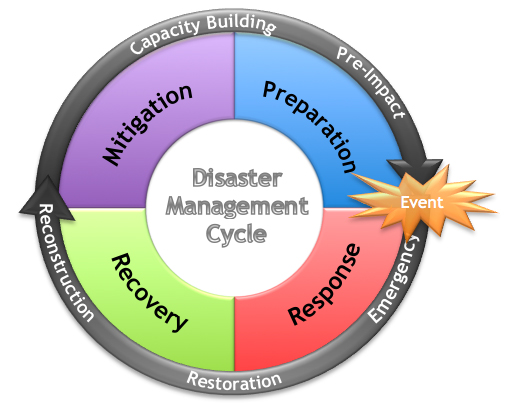
\includegraphics[width=1.00\textwidth]{graphics/Disaster_Capacity_Building.jpg}
	\caption{Disaster Management Cycle.  }
	\label{fig:Disaster_Capacity_Building}
\end{figure}

Since simulations are part of the PEER program, they focus on both hospitals and general community response. PEER’s 3-stage hospital simulation exercise includes (1) a tabletop-based exercise which forms the backbone of a multi-hazard response plan, (2) a functional command post exercise where the management team practices directing hospital response without actually deploying resources, and (3) a full-scale exercise that involves the Hospital Command Centre and deploys emergency personnel to manage patient reception at the emergency department (ADPC, 2015). To test community-based flood management plans initiated by the Talad Kao and Ban Buphram communities, PEER also conducted flood simulation exercises where trained CADRE volunteers practiced undertaking water rescue missions. Post-simulation, communities brainstormed for better interventions (ADPC, 2015).

Outside of PEER programs, schools have also been heavily involved in planning for flood safety where school-specific inputs from teachers and students were sourced and plans were integrated with existing resources and capacities of their wider community. For example, Wat Hua Hin school’s action plan was integrated with the Community Flood Preparedness Plan of Moo (village, subdivision of Tambon) 2, Ban Hua Hin, and Tha Luang TAO (Tambon (subdistrict) Administrative Organisation) (ADPC, 2015). Some schools have also agreed to share resources like evacuation space, such as Luang Wittayanukul and Wat Kai Jone (ADPC, 2015). The increased interaction between communities and local, provincial and national development institutions have both allowed for better coordination and integration of action plans and developed better understanding of how local water levels are influenced by upstream irrigation and water releases.

The involvement of community in decision-making has also facilitated the brainstorming of innovative ideas (Figure 14) such as using the ‘LINE’ mobile phone application to coordinate flood warning response, together with strategically placed loudspeakers and CCTVs (ADPC, 2015). Another example is the installation of water purification equipment. After community members in Ban Hua Hin identified water purification as a priority for reducing flood impact, the equipment was installed at a daycare centre where money collected from the machines (1 baht per litre) would contribute to the maintenance of the system, managed by the community-based flood management community (ADPC, 2015).  

Especially since the lack of real-time information on water and human conditions and on ‘who is doing what’ has been identified as a key information gap that contributed to the magnitude of the 2011 flood impacts (Jukrkorn et al., 2014), the improved coordination and integration that CBDRM brings is valuable. 

\begin{figure}[htbp]
	\centering
		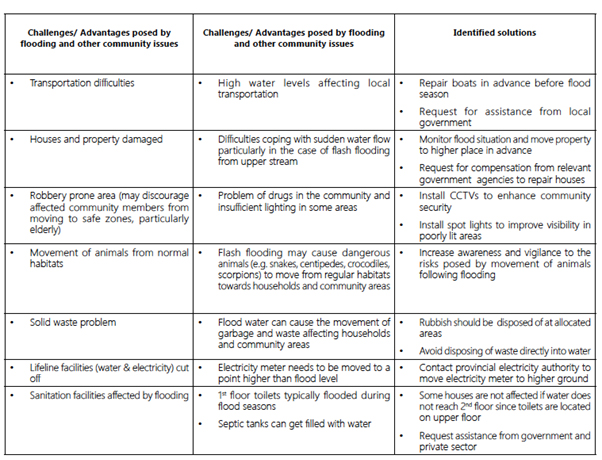
\includegraphics[width=1.00\textwidth]{graphics/CBDRM_Examples.jpg}
	\caption{Examples of CBDRM (for flood risk) planning materials and tools utilised in target communities  (Source: Asian Disaster Preparedness Center)}
	\label{fig:CBDRM_Examples}
\end{figure}



\section{Concluding Remarks}

In this chapter we have elaborated in detail upon the production of both hazards and vulnerabilities to floods and droughts in Thailand. We highlight that this production is complex and multi-dimensional, involving both natural conditions and political interventions by a range of actors. 

In the later half of this document, we then explored possible approaches towards more inclusive and resilient disaster risk reduction based on community involvement. Despite the forward-lookingness of the principles and ideologies we have mentioned, studies on their applications to flood and drought risk management in Thailand -- whether the SEP, Eco-DRR or CBDRM -- have been limited. 

Moving forward, it is important for research to evaluate the impact of existing community-based initiatives, most notably those of CBDRM. Studies should explore how individuals within communities perceive the effectiveness of these initiatives. While such research is currently scarce in the literature (Zwi et al., 2013), further studies would inform understandings of the benefits and disadvantages of such approaches, and the extent to which these initiatives have had an impact on the lives of the Thai people.


Statement of Contributions

All authors contributed equally to the paper in the form of research, writing, section editing and compilation of the bibliography and all sources. All authors were assigned to work on 2 chapters each. CL worked to put together the Introduction and Chapters 2 and 4. HJM worked to assemble Chapters 1, 2 and 6. JT worked on Chapters 3 and 5. NBC worked on Chapters 3 and 4. SKS worked on Chapters 5 and 6. JT worked on overall edits for style, language and logical flow to ensure consistency and comprehensibility of the final document.

